\chapter{機器學習}
\section{類神經網絡}
\begin{figure}[hbt!]
\begin{center}
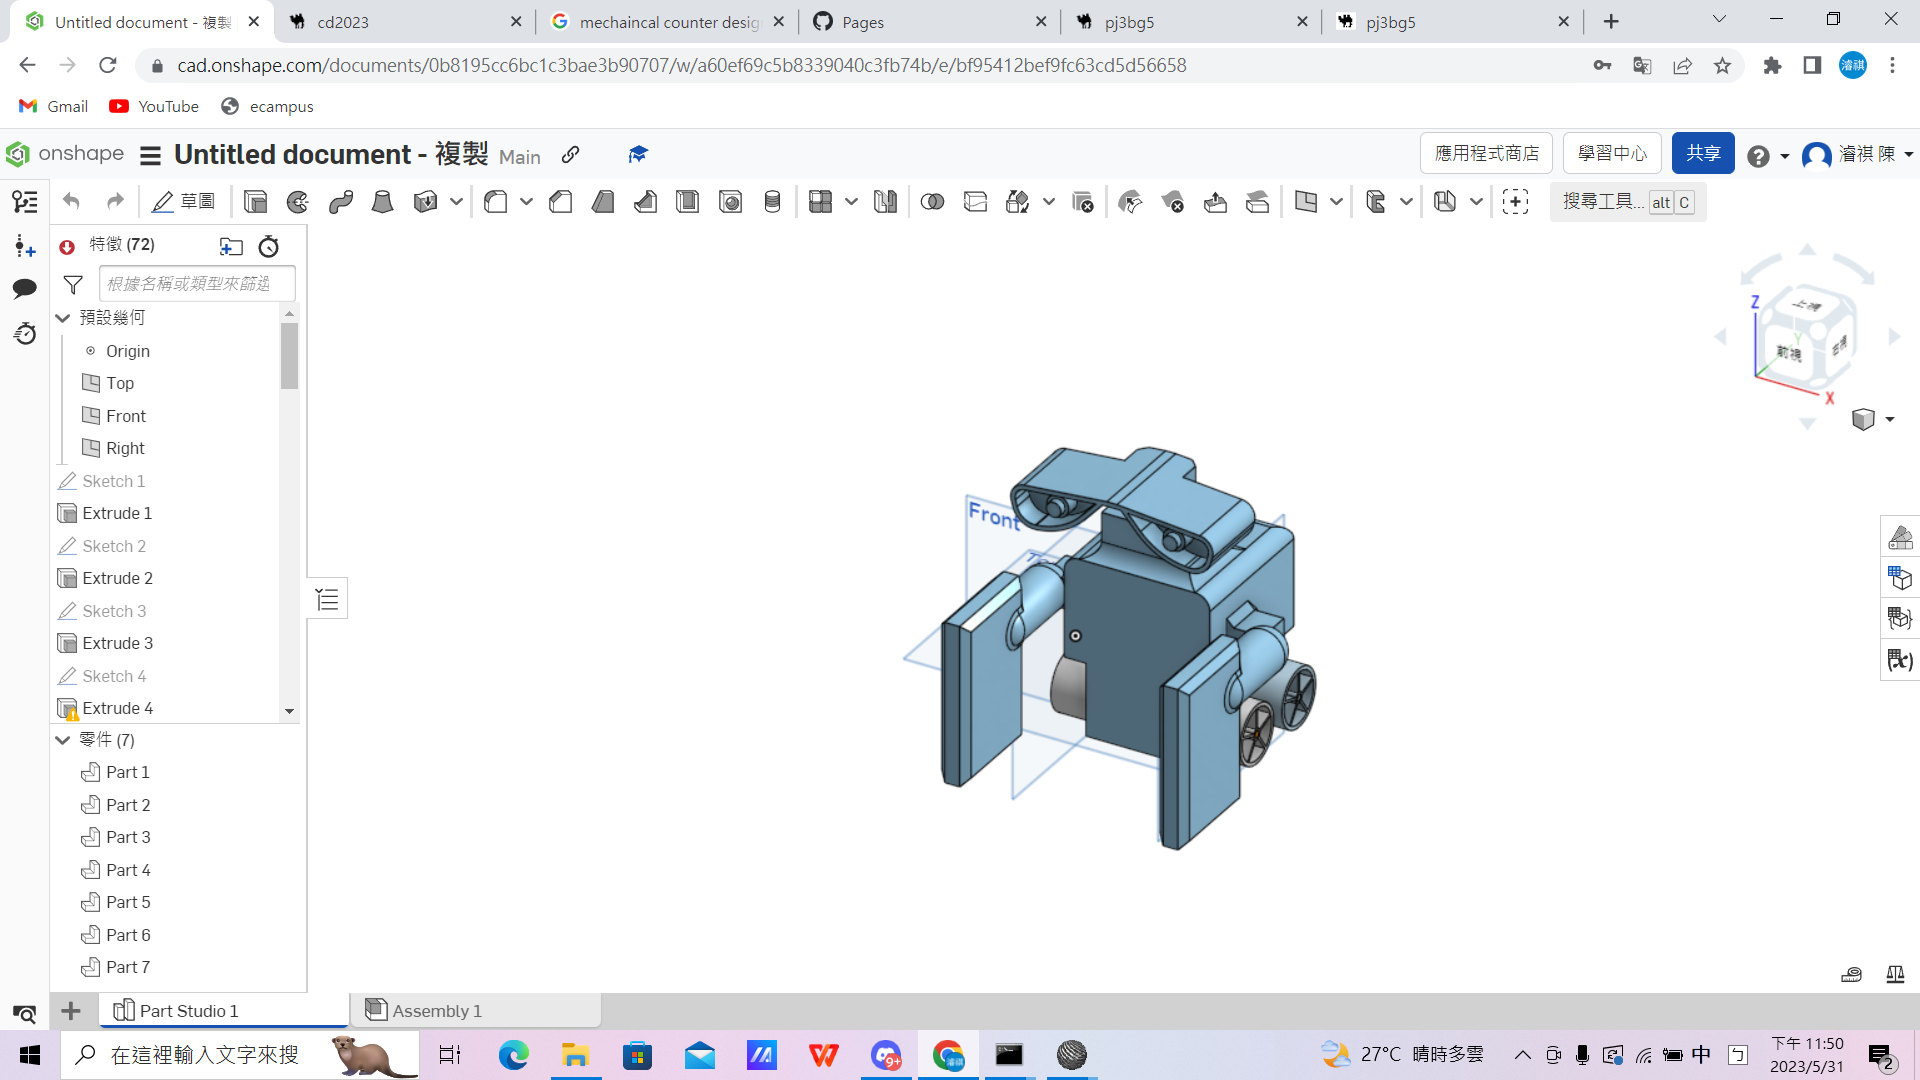
\includegraphics[width=16cm]{11111}
\caption{\Large 類神經網路架構}\label{類神經網路架構}
\end{center}
\end{figure}

 典型的類神經網路架構,如所示每一層的每一個神經元都會連接到下一層全部的神經元,對於每個神經元輸出會有不同的權重。\\

 神經元是AI系統中使用的數學模型,其行為與實際的大腦神經元運作方式相仿,模型以數字的方式表達,神經元間傳遞會有不同強度,而以數值的大小代表不同強度,這個數值我們稱為權重,對結果產生重要的影響。\\

 基礎的類神經網路架構主要由輸入層、隱藏層和輸出層這三部分組成,實際運用上還有更多樣更複雜的類神經網路架構,深度學習則是有更多的隱藏層,從意義上來說就是增加了類神經網路的深度。\\

 此外,如所示,資料由輸入層傳入,經過隱藏層運算和記憶,再由輸出層進行輸出,這種資料被傳遞的方式被稱為前饋輸入(feed-forward)。\\

 類神經網路架構有了記憶,就能進一步讓網路學習。當類神經網路接收資料並猜測答案,如果答案與實際答案不符、有落差或有錯誤的情況,它會回授並修改對每個神經元權重和偏差修正的程度,並嘗試調配各項數值來修正輸出的結果,讓結果的正確性提高,這樣的修正行為就被稱為反向傳播(back-propagation)。透過迭代方法進行反複試驗,模擬人們學習的行為,而每一次的迭代被稱為epoch,經過一定的迭帶次數後會透過反向傳播修正輸出的誤差,經過不斷執行的修正,最終類神經網路的學習會不斷進步並給出更好的答案,訓練時間長短取決於訓練項目的複雜程度。\\

 可以看到該神經網絡的輸出僅取決於互連的權重,還取決於神經元本身的偏差,雖然權重會影響啟動函數曲線的陡度,但是偏差會將發生變化的整個曲線,向右或向左,權重和偏差的選擇,決定了單個神經元的預測強度,而訓練類神經網絡使用的輸入數據可以來微調權重和偏差。\\

\newpage
\begin{figure}
\begin{center}
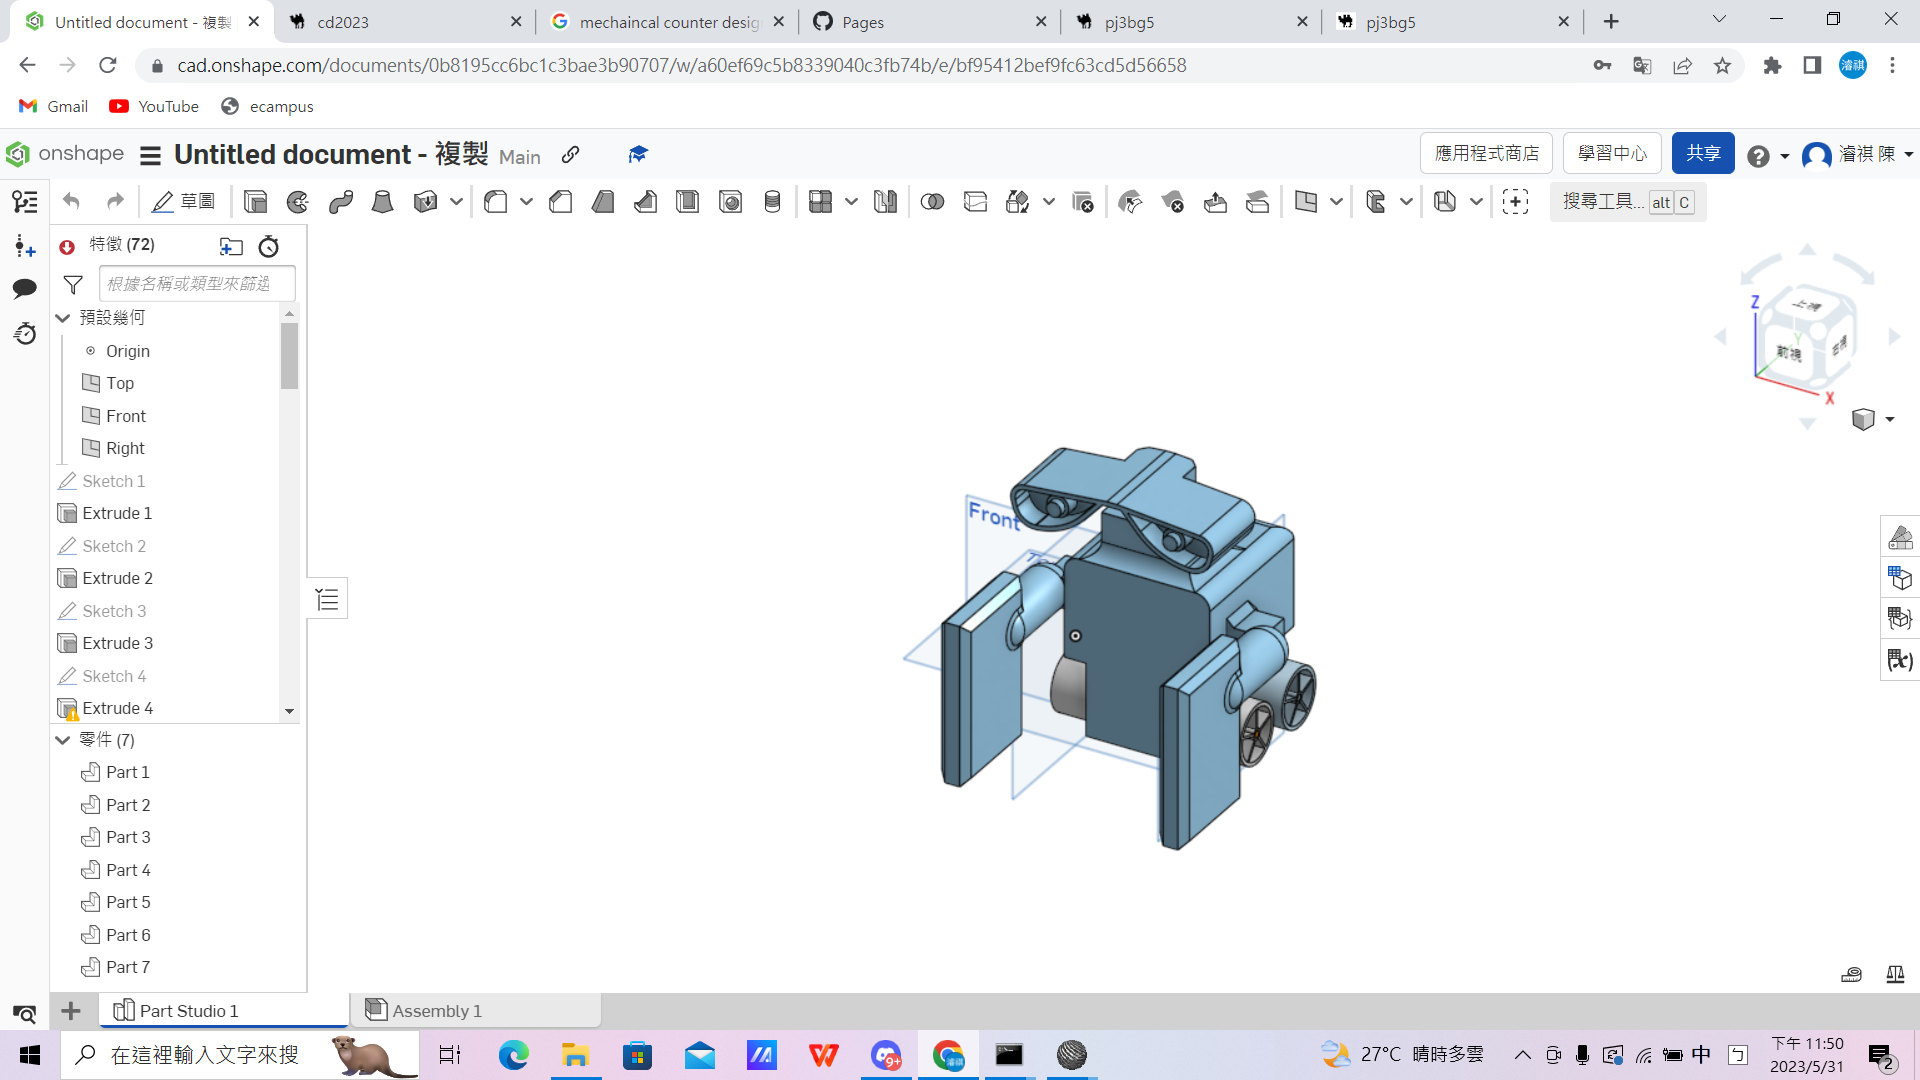
\includegraphics[width=16cm]{11111}
\caption{\Large 類神經網路關係}
\label{類神經網路關係}
\end{center}
\end{figure}
\subsection{啟動函數}
啟動函數是設計類神經網路的關鍵部分,如果不使用啟動函數,神經元的計算只會有線性組合,這樣的類神經網路缺乏活性而且記憶性差;啟動函數能讓神經元計算呈現非線性,讓類神經網路因為計算的非線性而提高整個網路的活性和記憶性。\\

\subsection{損失函數}
損失函數是類神經網路的另一個重要的部分,損失函數會將類神經網絡的結果與期望結果進行比較,且必須重複估算模型當前狀態的誤差;該函數可用於估計模型的損失,以便可以更新權重減少下次評估時的損失,下一節會有詳細說明,以下簡述幾種優化的方法:\\
\begin{itemize}
\item Gradient Descent\\
利用梯度的方式尋找最小值的位置,其特色可找到凸面error surface的絕對最小值,在非凸面error surface上找到相對最小值。其缺點是在非凸面error surface要避免被困在次優的局部最小值。
\item Batch gradient descent\\
用批次的方式計算訓練資料,整個資料集計算梯度只更新一次,因此計算和更新時會占用大量記憶體。整體效率較差、速度較緩慢。由 Gradient Descent 延伸出來的算法。其收斂行為與 Gradient Descent 相同。
\item Stochastic gradient descent\\
每次執行時會更新並消除誤差,有頻繁更新和變化大的特性,較不容易困在特定區域。由 Gradient Descent 延伸出來的算法。其收斂行為與 Gradient Descent 相同。
\item Mini-batch gradient descent\\
結合 Batch gradient descent 和 Stochastic gradient descent 的特點:批量計算和頻繁更新,所衍伸的算法。利用小批量的方式頻繁更新,並使收斂更穩定。其缺點:學習率挑選不易、預定義 threshold 無法適應數據集的特徵、對很少發生的特徵無法執行較大的更新、非凸面error surface要避免被困在次優的局部最小值等。
\item Gradient descent optimization algorithms\\
為了改善前面幾種算法而發展出來的優化算法。以下將列出數種優化算法。
\item Momentum\\
在梯度下降法加上動量的概念,會加速收斂到最小值並減少震盪。
\item Nesterov accelerated gradient\\
NAG,有感知能力的 Momentum:在坡度變陡時減速,避免衝過最小值所造成的震盪(為了修正到最小值,來回修正而產生的震盪)。
\item Adagrad\\
其學習率能適應參數:頻繁出現的特徵用較低的學習率,不經常出現的特徵則用較高的學習率,且無須手動調整學習率。其缺點是,學習率會急遽下降,最後會無限小,這算法就不再獲得知識。
\item Adadelta\\
為 Adagrad 的延伸,下降激進程度,學習率從更新規則中淘汰,不需設定預設學習率。
\item RMSprop\\
為了解決 Adagrad 學習率急劇下降的問題,學習率除以梯度平方的RMS,解決學習率無限小的情形。
\item Adam Function\\
結合了 Adagrad 和 RMSprop的優勢,有論文表示,在訓練速度方面有巨大性的提升,但在某些情況下,Adam實際上會找到比隨機梯度下降法更差的解決方法。以下是計算過程:\\
$$g_t=\delta_{\theta}f(\theta)$$
一次矩指數移動均線 :\\
$$m_t =\beta(m_{t-1})+(1-\beta_1)(\nabla{w_t})$$
$$\hat m_t=\frac{m_t}{1-\beta_1^t}$$
二次矩指數移動均線 :\\
$$v_t=\beta_2(v_t-1)+(1-\beta_2)(\nabla{w_t})^2$$
$$\hat{v_t}=\frac{v_t}{1-\beta_2^t}$$
因此,Adam Function:\\
$$\omega_{t-1}=\omega_t-\frac{\eta}{\sqrt{\hat{v_t}-\epsilon}}\hat{m_t}$$
\item AdaMax\\
與 Adam 相似,依靠$(u_t)$ 最大運算。
\item Nadam\\
結合 Adam 和 NAG ,應用先前參數執行兩次更新,一次更新參數一次更新梯度。
\item AMSGrad\\
改善 Adam 算法所導致收斂較差的情況(用指數平均會減少其影響),換用梯度平方最大值來做計算,並移除去偏差的步驟。是否有比 Adam 算法好仍有待觀察。
\item Gradient noise\\[6pt]
有助於訓練特別深且復雜的網絡,noise 可改善不良初始化的網路。
\item Mean Squared Error\\
他能告訴你一組點與回歸線接近的程度,透過獲取點與回歸線之距離(這些距離就是誤差)並對它們進行平方來做到這點,而平方是為了消除所有負號,也能讓更大的差異賦予更大的權重。\\
\vspace{8cm}
\end{itemize}
\newpage

\section{強化學習}
%=----------What is Reinforcement Learning?------------=%
強化學習(Reinforcement Learning,簡稱為RL)是通過agent(代理)與已知或未知的環境持續互動,不斷適應與學習,會得到正向或負面的回饋,對應到獎賞(reward)和懲罰(punishments)。考慮到agent與環境(environment)互動,進而決定要執行哪個動作,強化學習的學習模式是建立在獎賞與懲罰上。\\

強化學習與其他學習法不一樣的地方在於:不需要事先收集大量數據提供當作學習樣本,而是透過與環境互動,在環境下發生的狀態當作學習的資料來源,透過不斷嘗試使所得到的獎勵最大化。其他類型的機器學習大都需要給予特定資料且有明確的答案。\\

由於強化學習是建立在agent與環境互動上,因此許多參數進行運算,需要大量資訊來學習,並根據資訊採取行動。強化學習的環境可以是真實世界、2D或3D模擬世界的場景。強化學習的範圍很廣,因為環境的規模可能很大,且在環境中有多相關因素,影響著彼此。強化學習以獎勵的方式,促使學習結果趨近或達到目標結果。\\

\newpage
